\documentclass[aspectratio=169]{beamer}
\usepackage{fancyvrb}
\usepackage{framed}
\usepackage{caption}
\usepackage{qrcode}
\usetheme{CambridgeUS}

\usepackage{listings}
\usepackage{xcolor}
\usepackage{algorithm}
\usepackage{algpseudocode}
\usepackage{tikz}
\usepackage{marvosym} % for \Lightning

\newcommand{\sharpsat}{\ensuremath{\mathsf{sharpSAT}}}% NOTE: SharpSAT-TD but sharpSAT. YES!!
\newcommand{\sharpsattd}{\ensuremath{\mathsf{SharpSAT}}-\ensuremath{\mathsf{TD}}} % NOTE: SharpSAT-TD but sharpSAT. YES!!
\newcommand{\ganak}{\ensuremath{\mathsf{Ganak}}}
\newcommand{\exactmc}{\ensuremath{\mathsf{ExactMC}}}
\newcommand{\arjun}{\ensuremath{\mathsf{Arjun}}}
\newcommand{\dfour}{\ensuremath{\mathsf{d4}}}
\newcommand{\gpmc}{\ensuremath{\mathsf{gpmc}}}
\newcommand{\satisfying}[1]{\ensuremath{\mathsf{Sol}(#1)}}
\newcommand{\projectsatisfying}[2]{\ensuremath{\mathsf{Sol}(#1)_{\downarrow #2}}}
\newcommand{\toolname}{\ensuremath{\mathsf{Ganak2}}}
\def\checkmark{\tikz\fill[scale=0.2](0,.35) -- (.25,0) -- (1,.7) -- (.25,.15) -- cycle;} 
 \newcommand{\electricityArrow}{
 \tikz[scale=0.15]{ \draw[thick] (0,-1) -- (0.5,-1.5) -- (0,-2) -- (0.5,-2.5); \draw[thick, ->] (0.5,-2.5) -- (0.5,-3); } }
\newtheorem{observation}{Observation}
\algnotext{EndWhile}  % Suppresses "end while"
\algnotext{EndFor}    % Suppresses "end for"
\algnotext{EndIf}

\title[Engineering an Efficient Model Counter]{Engineering an Efficient Probabilistic Exact Model Counter}
\author[Soos, Meel]{Mate Soos, Kuldeep S. Meel}
\institute[UofT, GATech]{\large University of Toronto, Georgia Tech}
\date{24th of July 2025, Zagreb, CAV 2025}

\begin{document}
\begin{frame} \titlepage
\end{frame}

\begin{frame}{Outline}
    \tableofcontents
\end{frame}

\section{Propositional Model Counting}
\begin{frame}[fragile=singleslide]{Propositional Model Counting}
\begin{itemize}
  \item Count the number of solutions to a CNF, e.g $(x_1 \lor x_2) \land (\neg x_1 \lor x_3)$
  \item Notice that finding a single solution is in NP. Counting is \#P
  \item Sometimes, we project the solution space, like so:
  \begin{verbatim}
  Projection set | Other variables
  --------------------------------
  0001           |010111
  0001           |101010
  1011           |111010
  \end{verbatim} This problem only has 2 solutions over the projection set (but
  3 overall)
  \item Sometimes, literals in the projection set have a ``weight''
  \item Weight is usually a rational number, but it can be any element of
    a semiring
  \item Then, each solution has a ``weight'': the product of each literal's weight
  \item Final solution in this case is the sum of each solution's weight, i.e.
    \textbf{sum-of-products}
\end{itemize}
\end{frame}

\begin{frame}{Our Contributions to d-DNNF Model Counting}
\begin{columns}
\begin{column}{0.45\textwidth}
  We count solutions to the CNF by compiling the CNF into a \textbf{d-DNNF}{\color{blue}[Darwiche\&Marquis, 2002]}:
  a deterministic decomposable negation normal form circuit.
\end{column}
\begin{column}{0.55\textwidth}
\begin{center}
\scalebox{0.8}{
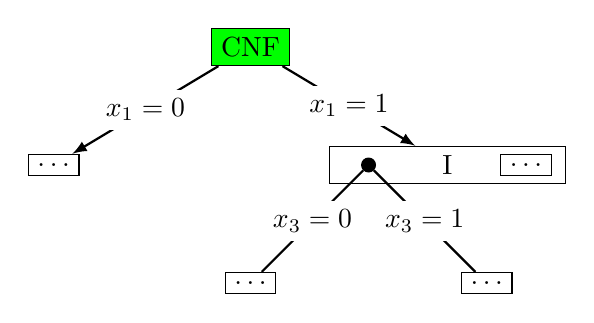
\begin{tikzpicture}[
    level distance=1.5cm,
    sibling distance=4cm,
    level 1/.style={sibling distance=5cm},
    level 2/.style={sibling distance=3cm},
    every node/.style={draw},
    edge from parent/.style={
        draw,
        ->, thick, >=latex,
        edge from parent path={(\tikzparentnode) -- (\tikzchildnode)}
    },
    edge from parent node/.style={draw=none},
    edge label/.style={fill=white, draw=none}
]
\tikzstyle{dot} = [circle, fill=black, minimum size=5pt, inner sep=0pt]
\tikzstyle{box} = [draw, minimum width=3cm, minimum height=2cm]
\tikzstyle{subgraph} = [draw, thick, circle, minimum size=1cm]
\node[fill=green] {CNF} 
child {
    node[fill=white] {$\ldots$}
    edge from parent node[edge label] {$x_1=0$}
}
child {
    node[style=rectangle, fill=white, minimum width=3cm] (mainbox) {I}
    edge from parent node[edge label] {$x_1=1$}
};

% Place dots inside the box 
\node[dot] (dot1) at ([xshift=-1cm]mainbox.center) {}; 
\node[] (dot2) at ([xshift=1cm]mainbox.center) {$\ldots$};

\node[](subgraph10) at ([yshift=-1.5cm, xshift=-1.5cm]dot1) {$\ldots$};
\node[] (subgraph11) at ([yshift=-1.5cm, xshift=1.5cm]dot1) {$\ldots$};

% Connect lines to subgraphs 
\draw[thick] (dot1) -- (subgraph10) node[midway,draw=none,fill=white] {$x_3=0$};
\draw[thick] (dot1) -- (subgraph11) node[midway,draw=none,fill=white] {$x_3=1$};
\end{tikzpicture} }
\end{center}
\end{column}
\end{columns}
\smallskip

\begin{enumerate}
  \item  \textbf{Enhanced Residual Formula Processing}: optimized SAT solver
    architecture for residual formula processing that incorporates VSIDS
    scoring, restarts, and polarity caching.
  \item \textbf{Dual Independent
    Set Framework}: maintains distinct SAT-eligibility (S) and decision (D)
    sets, where the S-set determines SAT solver transitions while the D-set
    guides branching decisions.
  \item \textbf{Chronological Backtracking}:
    Adaptation of chronological backtracking to model counting
\end{enumerate}
\end{frame}

\section{Our Enhancements}
\begin{frame}{Calling a SAT solver}
\begin{columns}
\begin{column}{0.42\textwidth}
Once all variables in $P$ have been decided there is only one solution: we can run a SAT solver!
\bigskip

$V=\{x_1, x_2, x_3, x_4, \ldots \}$

$P=\{x_1, x_2\}$
\bigskip

Once $\{x_1, x_2\}$ have all been branched on, we can call a SAT solver on the residual formula!
\bigskip

\bigskip

This has been exploited before by \gpmc{}
\end{column}
\begin{column}{0.58\textwidth}
\begin{center}
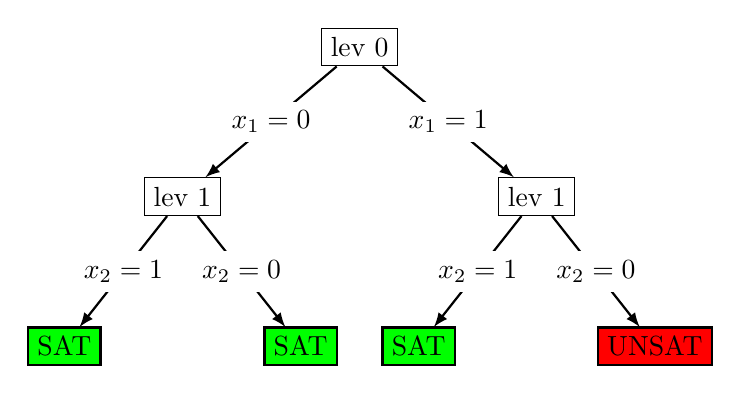
\begin{tikzpicture}[
	level distance=1.9cm,
	sibling distance=4.5cm,
	level 2/.style={sibling distance=3cm},
	every node/.style={draw},
	edge from parent/.style={
		draw,
		->, thick, >=latex,
		edge from parent path={(\tikzparentnode) -- (\tikzchildnode)}
	},
	edge from parent node/.style={draw=none},
	edge label/.style={fill=white, draw=none}
	]
	\node[fill=white] {lev 0} 
	child {
		node[fill=white] {lev 1}
		child {
			node[minimum size=0.3cm,fill=green] {SAT}
			edge from parent node[edge label] {$x_2=1$}
		}
		child {
			node[minimum size=0.3cm,fill=green] {SAT}
			edge from parent node[edge label] {$x_2=0$}
		}
		edge from parent node[edge label] {$x_1=0$}
	}
	child {
		node[fill=white] {lev 1}
		child {
			node[minimum size=0.3cm,fill=green] {SAT}
			edge from parent node[edge label] {$x_2=1$}
		}
		child {
			node[minimum size=0.3cm,fill=red] {UNSAT}
			edge from parent node[edge label] {$x_2=0$}
		}
		edge from parent node[edge label] {$x_1=1$}
	};
\end{tikzpicture}
\end{center}
\end{column}
\end{columns}
\end{frame}

\begin{frame}{Enhanced Residual Formula Processing}
We added:
\begin{itemize}
  \item \textbf{VSIDS Scoring}: Model counters use VSADS\footnote{\color{blue}Variable State Aware Decaying Sum, from Sang et al.'05} scoring, but for
      SAT, VSIDS is faster to compute, and more efficient.
    \item \textbf{Restarts}: Restart the SAT solver regularly (Luby
      heuristic\footnote{\color{blue}Luby et al, '93}), to
      explore different parts of the search space. Note we only need one
      solution.
    \item \textbf{Polarity Caching}\footnote{\color{blue}Pipatsrisawat et al, '07}: We cache the polarity of variables to
      avoid unnecessary recomputation, especially due to restarts
\end{itemize}
\bigskip

Basically: let's lift all the SAT techniques to model counting's residual formula processing.
\end{frame}

\begin{frame}{Dual Independent Set}
\begin{definition}[Dual Independent Set]
Given a Boolean formula $F$ defined over variables $V$ and a projection set
$\mathcal{P}$, a dual independent set consists of:
\begin{enumerate}
  \item \textbf{S-set} A SAT-eligibility set $S\subseteq \mathcal{P}$ that
    determines when SAT solver mode transition is permissible.
    \item \textbf{D-set} A decision set $D\subseteq V$ that guides branching
      variable selection, where $D \supseteq \mathcal{P}$.
\end{enumerate}
This formulation generalizes traditional approaches where $D = S \subseteq P$,
instead aiming for $S \subseteq P \subseteq D$.
\end{definition}
\bigskip

{
\begin{center}
  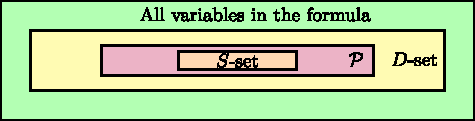
\includegraphics[scale=0.99]{figs/vars_fig.pdf}
\end{center}
}
\end{frame}

\begin{frame}{Computing Maximal Decision Set}
  \small
  \begin{algorithmic}[1]
    %\Require Formula $F$, projection set $\mathcal{P}$
    %\Ensure Maximal decision set $D_{\text{max}}$ where $\mathcal{P} \subseteq D_{\text{max}}$
    
    \State $D \gets \mathcal{P}$,  $G \gets \textsc{ExtractGates}(F)$ \Comment{Initialize $D$ with $\mathcal{P}$, Extract gates}
    
    \Procedure{SyntacticExpansion}{$V$}
    \State $\text{changed} \gets V$
    \While{changed is not empty} 
    \State $v \gets \text{changed}.pop()$
    \For{gate $g \in G$ where $v$ is input} If possible, extend $D$ with output of the gate
    \EndFor
    \EndWhile
    \State \Return $D$
    \EndProcedure
    
    \Procedure{SemanticExpansion}{}
    \For{$v \notin D$}
    \If{$\textsc{ValidateDecisionVar}(D \cup \{v\}, F)$}
        \State $D \gets D \cup \{v\}$
        \State $D \gets \textsc{SyntacticExpansion}(\{v\})$\Comment{Quick check with syntactic analysis}
    \EndIf
    \EndFor
    \State \Return $D$
    \EndProcedure

    % \State $D \gets \textsc{SyntacticExpansion}(P)$ \Comment{Phase 1: Syntactic analysis}
    % \State $D \gets \textsc{SemanticExpansion}$ \Comment{Phase 2: Semantic analysis}
    % \State \Return $D$
  \end{algorithmic}
We run $\textsc{SyntacticExpansion}(P)$ and then $\textsc{SemanticExpansion}$
\end{frame}

\begin{frame}{Chronological Backtracking}
Notice that we should NOT backjump or we lose already counted solutions.
\begin{columns}
\begin{column}{0.45\textwidth}
  \small
\begin{itemize}
  \item Model counters go back to the deepest level possible, flip the
    decision, and throw away the learnt clause in case it would violate
    propagation invariants
  \item But we can relax some of the invariants: Chronological Backtracking
    (ChronoBT)
  \item ChronoBT allows the have out-of-order implication levels in the
    trail
% \begin{itemize}
  \item ChronoBT allows us to keep the learnt clause, and force
    the literal that the learnt clause entails.
  \item We used the fuzzer \texttt{SharpVelvet} by Latour et al. to find bugs
    in our implementation
% \end{itemize}
\end{itemize}
\end{column}
\begin{column}{0.55\textwidth}
\begin{center}
  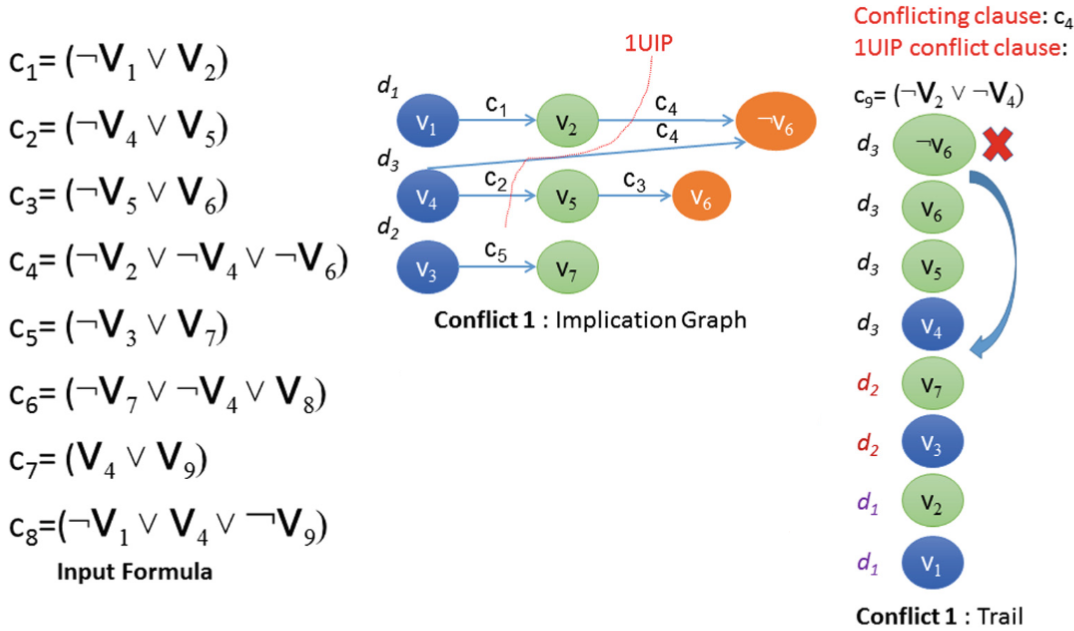
\includegraphics[scale=0.9]{chronoBT.png}
  \small Figure from \color{blue}Chronological Backtracking by Nadel\&Ryvchin, 2018
\end{center}
\end{column}
\end{columns}
\end{frame}

\begin{frame}{Compensating Weights}
\begin{columns}
\begin{column}{0.45\textwidth}
  \small
  \begin{enumerate}
  \item We explore the left side of a graph, nodes 1 and 2
  \item We backtrack to level $0$ and explore the right side, nodes 3 and 4.
  \item At node 4, we find the unit clause $x_3$. This unit clause's
  level is 0, but due to ChronoBT, we only backtrack to level 1. However,
  the system \textbf{has already multiplied in the weight of $\mathbf{x_3}$} into nodes
  1, 2, and 3.
\item These nodes' weights, which on the left side of an already 
  explored branch need to be compensated
\end{enumerate}
\end{column}
\begin{column}{0.55\textwidth}
\begin{center}
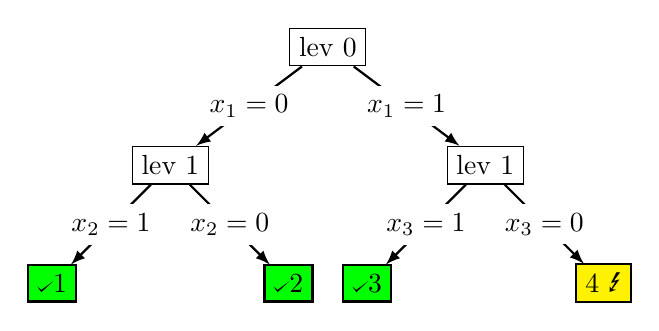
\begin{tikzpicture}[
	level distance=1.5cm,
	sibling distance=4cm,
	level 2/.style={sibling distance=3cm},
	every node/.style={draw},
	edge from parent/.style={
		draw,
		->, thick, >=latex,
		edge from parent path={(\tikzparentnode) -- (\tikzchildnode)}
	},
	edge from parent node/.style={draw=none},
	edge label/.style={fill=white, draw=none}
	]
	\node[fill=white] {lev 0} 
	child {
		node[fill=white] {lev 1}
		child {
			node[minimum size=0.3cm,fill=green] {$\checkmark 1$}
			edge from parent node[edge label] {$x_2=1$}
		}
		child {
			node[minimum size=0.3cm,fill=green] {$\checkmark 2$}
			edge from parent node[edge label] {$x_2=0$}
		}
		edge from parent node[edge label] {$x_1=0$}
	}
	child {
		node[fill=white] {lev 1}
		child {
			node[minimum size=0.3cm,fill=green] {$\checkmark 3$}
			edge from parent node[edge label] {$x_3=1$}
		}
		child {
			node[minimum size=0.3cm,fill=yellow] {4 \Lightning}
			edge from parent node[edge label] {$x_3=0$}
		}
		edge from parent node[edge label] {$x_1=1$}
	};
\end{tikzpicture}
\end{center}
\end{column}
\end{columns}
\end{frame}

\begin{frame}{Compensating Weights}
\begin{columns}
\begin{column}{0.45\textwidth}
\begin{enumerate}
\small
\item $x_4$ is part of components \{1,2,3,4\} but not 5
  is learned to be false at level 0.
\item Sounds impossible. $x_4$ is clearly not part of component 5
  (since it is part of 3 and 4), so it should never be part of a learned clause
  while examining component 5
\item Components are decided \emph{purely} based on irredundant
  clauses. It is possible that learned clauses connect components!
\item Can lead to contradictions over variables \emph{not} part of the
  component examined!
\item Compensating for these is non-trivial: \emph{sibling} components
  need to be examined and compensated for
\end{enumerate}
\end{column}
\begin{column}{0.55\textwidth}
\begin{center}
\scalebox{0.8}{
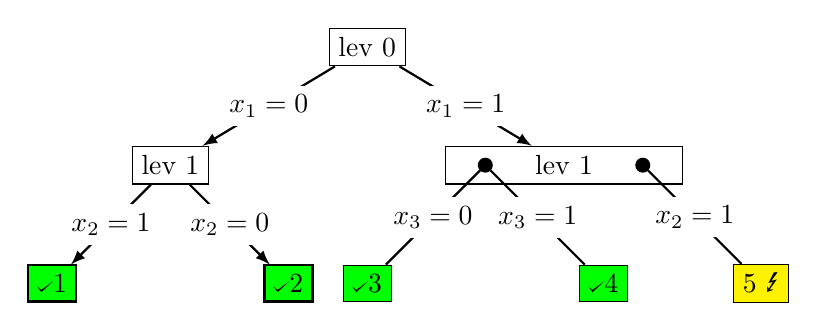
\begin{tikzpicture}[
    level distance=1.5cm,
    sibling distance=4cm,
    level 1/.style={sibling distance=5cm},
    level 2/.style={sibling distance=3cm},
    every node/.style={draw},
    edge from parent/.style={
        draw,
        ->, thick, >=latex,
        edge from parent path={(\tikzparentnode) -- (\tikzchildnode)}
    },
    edge from parent node/.style={draw=none},
    edge label/.style={fill=white, draw=none}
]
\tikzstyle{dot} = [circle, fill=black, minimum size=5pt, inner sep=0pt]
\tikzstyle{box} = [draw, minimum width=3cm, minimum height=2cm]
\tikzstyle{subgraph} = [draw, thick, circle, minimum size=1cm]
\node[fill=white] {lev 0} 
child {
    node[fill=white] {lev 1}
    child {
        node[minimum size=0.3cm,fill=green] {$\checkmark 1$}
        edge from parent node[edge label] {$x_2=1$}
    }
    child {
        node[minimum size=0.3cm,fill=green] {$\checkmark 2$}
        edge from parent node[edge label] {$x_2=0$}
    }
    edge from parent node[edge label] {$x_1=0$}
}
child {
    node[style=rectangle, fill=white, minimum width=3cm] (mainbox) {lev 1}
    edge from parent node[edge label] {$x_1=1$}
};

% Place dots inside the box 
\node[dot] (dot1) at ([xshift=-1cm]mainbox.center) {}; 
\node[dot] (dot2) at ([xshift=1cm]mainbox.center) {};

\node[fill=green](subgraph10) at ([yshift=-1.5cm, xshift=-1.5cm]dot1) {$\checkmark 3$};
\node[fill=green] (subgraph11) at ([yshift=-1.5cm, xshift=1.5cm]dot1) {$\checkmark 4$};
\node[fill=yellow] (subgraph2) at ([yshift=-1.5cm, xshift=1.5cm]dot2) {5  \Lightning};

% Connect lines to subgraphs 
\draw[thick] (dot1) -- (subgraph10) node[midway,draw=none,fill=white] {$x_3=0$};
\draw[thick] (dot1) -- (subgraph11) node[midway,draw=none,fill=white] {$x_3=1$};
\draw[thick] (dot2) -- (subgraph2) node[midway,draw=none,fill=white] {$x_2=1$};
\end{tikzpicture} }
\end{center}
\end{column}
\end{columns}
\end{frame}

\begin{frame}{Compensating Weights}
\begin{itemize}
  \item Notice that to compensate we need to \textbf{divide}
  \item But weighted counting can be done with weights over any \textbf{semiring}
  \item But \toolname{} needs a \textbf{field}
  \item In some sense, we reorder computations, exploiting flexibility
    in building the d-DNNF
  \item Side-note: Ganak2 supports \textbf{any field}. Implementing a new
    field should take $\approx10$ minutes. Currently supports:
    \begin{itemize}
      \item Integers
      \item Counting modulo prime
      \item Rational numbers
      \item Floating point -- not a field actually
      \item Complex rational numbers
      \item Multivariate polynomials over the rationals
  \end{itemize}
\end{itemize}
\end{frame}

\section{Results}
\begin{frame}{Ganak Versions over all Instances}
  \begin{center}
    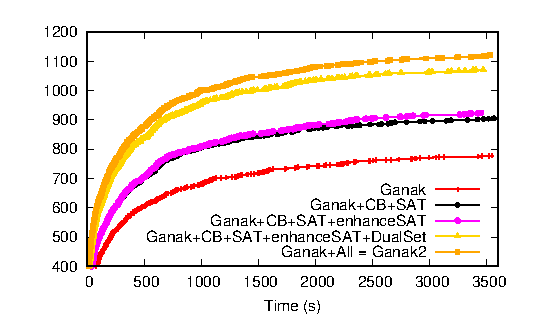
\includegraphics[scale=1.40]{figs/ganak-versions/run}
\end{center}
\end{frame}

\begin{frame}{All Instances, All Solvers}
  \begin{center}
  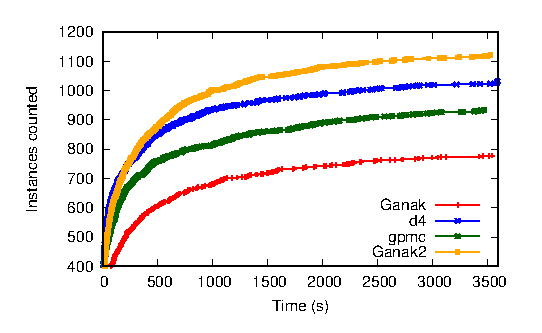
\includegraphics[scale=1.40]{figs/proj-and-unproj/run}
\end{center}
\end{frame}

\begin{frame}{Conclusions}
We created a new probabilistically exact model counter, \toolname{}, that incorporates:
\begin{itemize}
  \item \textbf{Enhanced Residual Formula Processing}
  \item \textbf{Dual Independent Set Framework}
  \item \textbf{Chronological Backtracking}
\end{itemize}

This allowed us to achieve state-of-the-art performance. \toolname{} won 
all tracks of the Model Counting Competition 2024.
\bigskip

\begin{center}
Code: \qrcode{https://github.com/meelgroup/ganak/}
\qquad \qquad
Paper: \qrcode{https://www.msoos.org/wordpress/wp-content/uploads/2025/05/ganak2.pdf}
\bigskip

Also, try it out online: \url{https://www.msoos.org/ganak/}
\end{center}
\end{frame}
\end{document}
